
% !BIB program = bibtex
%% --
%% -- LN-book-mult 
%% -- Stand: 2024/01/24
%% -- 

\documentclass[%
	,graybox
	,envcountchap]{svmult}

% choose options for [] as required from the list
% in the Reference Guide

%\usepackage{type1cm}        % activate if the above 3 fonts are 
                             % not available on your system

\usepackage{makeidx}         % allows index generation
\usepackage{graphicx}        % standard LaTeX graphics tool
                             % when including figure files
\usepackage{multicol}        % used for the two-column index
\usepackage[bottom]{footmisc}% places footnotes at page bottom

\usepackage{newtxtext}       % 
\usepackage[varvw]{newtxmath}       % selects Times Roman as basic font

% see the list of further useful packages in the Reference Guide

\makeindex             % used for the subject index
                       % please use the style svind.ist with
                       % your makeindex program
                       
%% -- Referenzen
%% --
\bibliographystyle{spmpsci}

%% -- LN Speziell
%% --
\usepackage[english]{babel}
\usepackage{csquotes}
\usepackage[inline,shortlabels]{enumitem}
\setlist{%
	,labelsep=0.8em
	,leftmargin=1em
	,itemindent=2em
	,labelwidth=10pt
	,itemsep=0.15ex
	,parsep=.75ex
	}
\usepackage{ragged2e}

%% -- Part A etc
%% -- A-I etc für \chapter
%% -- 1. für \section etc
%% --
\renewcommand\thepart{\Alph{part}}
\renewcommand\thechapter{\thepart-\Roman{chapter}}
\renewcommand\thesection{\arabic{section}}
\renewcommand\thesubsection{\thesection.\arabic{subsection}}

%% -- Wegen Überlappung im TOC
%\usepackage{tocloft}
%\renewcommand\cftchapnumwidth{1cm}

%% -- \subsection nicht ins TOC
%% --
\setcounter{tocdepth}{1}

%% -- Durchgehende Nummerierung
%% -- entbehrlich
\makeatletter
\let\c@remark=\c@theorem 		% Make remark share the theorem counter
\let\c@definition=\c@theorem 	% Make definition share the theorem counter
\let\c@example=\c@theorem 		% Make example share the theorem counter
\let\c@lemma=\c@theorem 		% Make lemma share the theorem counter
\let\c@corollary=\c@theorem 	% Make corollary share the theorem counter
\let\c@proposition=\c@theorem 	% Make proposition share the theorem counter
\let\c@remark=\c@theorem 		% Make proposition share the theorem counter
\let\c@remarks=\c@theorem 		% Make proposition share the theorem counter
\makeatother

%% -- Nummer von Theorem etc. korrekt
%% --
\newtheorem{remarks}[theorem]{Remarks}
\renewcommand\thetheorem{\thesection.\arabic{theorem}}
\renewcommand\theproposition{\thesection.\arabic{proposition}}
\renewcommand\thedefinition{\thesection.\arabic{definition}}
\renewcommand\thelemma{\thesection.\arabic{lemma}}
\renewcommand\thecorollary{\thesection.\arabic{corollary}}
\renewcommand\theremark{\thesection.\arabic{remark}}
\renewcommand\theremarks{\thesection.\arabic{remarks}}
\renewcommand\theexample{\thesection.\arabic{example}}
%% --

%% -- Definitionen -> muss richtig gemacht  werden
\DeclareMathOperator{\Id}{Id}
% !BIB program = %\newcommand{\WA}{$\mathrm{W}^{*}$}
%\newcommand{\CA}{$\mathrm{C}^{*}$}
%\newcommand{\Fix}{\mathrm{Fix}}

\usepackage{ablatt-defn}
\newcommand{\rank}{\mathrm{Rang}\,}

%% -- Stand
%% --

\date{Stand: \today}

%% --
\begin{document}

%% -- Titelseite
%% --
%\author{Wolfgang Arendt, Annette Grabosch, G\"unther Greiner, Ulrich Groh, Heinrich P. Lotz, Ulrich Moustakas, Rainer Nagel, Frank Neubrander, Ulf Schlotterbeck}
%%% --
%\title{One-parameter Semigroups of Positive Operators\\
%		{\large{Edited by R. Nagel}}}
%%% --
%\subtitle{Lecture Notes in Mathematics\\ \\ 1184\\ \\Springer-Verlag\\ Berlin Heidelberg New York Tokyo}
%%% --


\maketitle

\frontmatter%%%%%%%%%%%%%%%%%%%%%%%%%%%%%%%%%%%%%%%%%%%%%%%%%%%%%%

% !TEX root = ../LN-Book.tex
%%%%%%%%%%%%%%%%%%%%%%% dedic.tex %%%%%%%%%%%%%%%%%%%%%%%%%%%%%%%%%
%
% dedication
% Stand: 2025/01/13 ulgr
% Use this file as a template for your own input.
%
%%%%%%%%%%%%%%%%%%%%%%%% Springer %%%%%%%%%%%%%%%%%%%%%%%%%%

\begin{dedication}
{\RaggedRight\Large 
This second edition of \emph{One-Parameter Semigroups of Positive Operators} is dedicated to the memory 	of our 
co-authors, Heinrich P.~Lotz (1934--2010) and Ulf Schlotterbeck (1941--2021). 
Their contributions to the first edition remain an inspiration to us all. 
We miss their presence and remain grateful for the legacy they have left in this work.}
\end{dedication}





%%%%%%%%%%%%%%%%%%%%%%%foreword.tex%%%%%%%%%%%%%%%%%%%%%%%%%%%%%%%%%
% sample foreword
%
% Use this file as a template for your own input.
%
%%%%%%%%%%%%%%%%%%%%%%%% Springer %%%%%%%%%%%%%%%%%%%%%%%%%%

\foreword

%% Please have the foreword written here
Use the template \textit{foreword.tex} together with the document class SVMono (monograph-type books) or SVMult (edited books) to style your foreword\index{foreword}. 

The foreword covers introductory remarks preceding the text of a book that are written by a \textit{person other than the author or editor} of the book. If applicable, the foreword precedes the preface which is written by the author or editor of the book.


\vspace{\baselineskip}
\begin{flushright}\noindent
Place, month year\hfill {\it Firstname  Surname}\\
\end{flushright}


% !TEX root = ../LN-Book.tex
%%%%%%%%%%%%%%%%%%%%%%preface.tex%%%%%%%%%%%%%%%%%%%%%%%%%%%%%%%%%%%%%%%%%
% preface
% 2025/03/17 ulgr
%
%%%%%%%%%%%%%%%%%%%%%%%% Springer %%%%%%%%%%%%%%%%%%%%%%%%%%

\preface

\section*{Preface to the Revised First Edition}
	
	When the first edition of these lecture notes appeared in 1986, the theory of one-parameter semigroups of positive operators was undergoing rapid development, stimulated by applications in ergodic theory, evolution equations, stochastics, and mathematical physics. 
	Our goal at the time was to provide a systematic and accessible account of the foundations and structure theory of positive semigroups, with particular emphasis on Banach lattices and \CA-algebras.
	We were gratified by the positive reception the volume received and the extent to which it found use in research and graduate instruction.
	
	Over the past four decades, the mathematical community has continued to draw on the results and techniques developed in these notes. 
	Despite the appearance of newer texts and the evolution of the field, this volume has remained widely cited and used—likely due to its thorough and methodical treatment of a core area in functional analysis. 
	The sustained interest from both researchers and students has encouraged us to prepare this revised first edition.
	
	We have preserved the structure and exposition of the original edition but have made a number of editorial improvements, including transferring the entire book into \LaTeX{}. 
	Obvious misprints have been corrected, references and the subject index have been updated where appropriate, and the notes at the end of each chapter have been expanded to some subsequent developments. 
	However, we have refrained from substantially altering the original content in order to retain the historical character and coherence of the text.
	
	We gratefully acknowledge the efforts of our co-author, Ulrich Groh, who guided the transfer of the manuscript into \LaTeX{}, with the assistance of Klaus-Georg Kuhn and the support of Claude, an artificial intelligence model developed by Anthropic.
	
	It is our hope that this revised edition will continue to serve as a valuable resource for those working in operator theory, functional analysis, and their many applications. 
	We remain deeply grateful to our colleagues and readers who have provided feedback and encouragement over the years.
%% --
%\begin{quote}
%{\itshape
%This second edition of \emph{One-Parameter Semigroups of Positive Operators} is dedicated to the memory 	of our 
%co-authors, Heinrich P.~Lotz (1934--2010) and Ulf Schlotterbeck (1941--2021). 
%Their contributions to the first edition remain an inspiration to us all. 
%We miss their presence and remain grateful for the legacy they have left in this work.}
%\end{quote}
%% --
%\vspace{.75em}
%{\RaggedLeft{The authors} }


%% Please write your preface here

\section*{Preface to the First Edition}

As early as 1948 in the first edition of his fundamental treatise on \emph{Semigroups and Functional Analysis}, E.~Hille expressed the need for 

\begin{quote}
\textit{\ldots developing an adequate theory of transformation semigroups operating in partially ordered spaces} (l.c., Foreword). 
\end{quote}

In the meantime the theory of one-parameter semigroups of positive linear operators has grown continuously. 
Motivated by problems in probability theory and partial differential equations W.~Feller (1952) and R.~S.~Phillips (1962) laid the first cornerstones by characterizing the generators of special positive semigroups. 
In the 60's and 70's the theory of positive operators on ordered Banach spaces was built systematically and is well documented in the monographs of H.~H.~Schaefer (1974) and A.~C.~Zaanen (1983). 
But in this process the original ties with the applications and, in particular, with initial value problems were at times obscured. 
Only in recent years an adequate and up-to-date theory emerged, largely based on the techniques developed for positive operators and thus recombining the functional analytic theory with the investigation of Cauchy problems having positive solutions to each positive initial value. 
Even though this development --- in particular with respect to applications to concrete evolution equations in transport theory, mathematical biology, and physics --- is far from being complete, the present volume is a first attempt to shape the multitude of available results into a coherent theory of one-parameter semigroups of positive linear operators on ordered Banach spaces.

The book is organized as follows.
We concentrate our attention on three subjects of semigroup theory: \emph{characterization}, \emph{spectral theory} and \emph{asymptotic behavior}. 
By \emph{characterization}, we understand the problem of describing special properties of a semigroup, such as positivity, through the generator. 
By \emph{spectral theory} we mean the investigation of the spectrum of a generator. 
\emph{Asymptotic behavior} refers to the orbits of the initial values under a given semigroup and phenomena such as stability.

This program (characterization, spectral theory, asymptotic behavior) is worked out on four different types of underlying spaces.
\newpage
%% --
\begin{enumerate}[label=(\Alph*)]
\item 
On Banach spaces---Here we present the background for the subsequent discussions related to order.

\item 
On spaces $C_{0}(X)$ ($X$ locally compact), which constitute an important class of ordered Banach spaces and where our results can be presented in a form which makes them accessible also for the non-expert in order-theory.

\item 
On Banach lattices, which admit a rich theory and are still sufficiently general as to include many concrete spaces appearing in analysis; e.g., $C_0(X)$, $\mathcal{L}^p(k)$ or $l^p$.

\item 
On non-commutative operator algebras such as \CA- or \WA-algebras, which are not lattice ordered but still possess an interesting order structure of great importance in mathematical physics.

\end{enumerate}
%% --
In each of these cases we start with a short collection of basic results and notations, so that the contents of the book may be visualized in the form of a $4 \times 4$ matrix in a way which will allow \enquote{row readers} (interested in semigroups on certain types of spaces) and \enquote{column readers} (interested in certain aspects) to find a path through the book corresponding to their interest.

We display this matrix, together with the names of the authors contributing to the subjects defined through this scheme.
%% --
%\definecolor{darkgreen}{rgb}{0.0, 0.75, 0.0}
%\begin{table}[ht]
%\centering
%\begin{tabular}{l|c|c|c|c|}
%\cline{2-5}
% & \color{darkgreen}{I} & II & \color{darkgreen}{III} & IV \\
% & \color{darkgreen}{Basic} & Characterization & \color{darkgreen}{Spectral} & Asymptotics \\
% & \color{darkgreen}{Results} &  & \color{darkgreen}{Theory} & \\
%\hline
%\multicolumn{1}{|l|}{A. Banach} & R. Nagel & W. Arendt & G. Greiner & F. Neubrander \\
%\multicolumn{1}{|l|}{Spaces} & U. Schlotterbeck & H. P. Lotz & R. Nagel & \\
%\hline
%\multicolumn{1}{|l|}{B. $C_0(X)$} & R. Nagel & W. Arendt & G. Greiner & A. Grabosch \\
%\multicolumn{1}{|l|}{} & U. Schlotterbeck & & & G. Greiner \\
%\multicolumn{1}{|l|}{} & & & & U. Moustakas \\
%\multicolumn{1}{|l|}{} & & & & F. Neubrander \\
%\hline
%\multicolumn{1}{|l|}{C. Banach} & R. Nagel & G. Arendt & G. Greiner & A. Grabosch \\
%\multicolumn{1}{|l|}{Lattices} & U. Schlotterbeck & & & G. Greiner \\
%\multicolumn{1}{|l|}{} & & & & U. Moustakas \\
%\multicolumn{1}{|l|}{} & & & & R. Nagel \\
%\multicolumn{1}{|l|}{} & & & & F. Neubrander \\
%\hline
%\multicolumn{1}{|l|}{\color{darkgreen}{D. Operator}} & U. Groh & U. Groh & U. Groh & U. Groh \\
%\multicolumn{1}{|l|}{\color{darkgreen}{Algebras}} & & & & \\
%\hline
%\end{tabular}
%\end{table}
%% --
%\definecolor{darkgreen}{rgb}{0.0, 0.75, 0.0}
%\begin{table}[ht]
%\centering
%\begin{tabular}{l|c|c|c|c|}
%\cline{2-5}
% & I & II & III & IV \\
% & Basic & Characterization & Spectral & Asymptotics \\
% & Results &  & Theory & \\
%\hline
%\multicolumn{1}{|>{\columncolor{darkgreen}}l|}{A. Banach} & {R. Nagel} & W. Arendt & G. Greiner & F. Neubrander \\
%\multicolumn{1}{|>{\columncolor{darkgreen}}l|}{Spaces} & U. Schlotterbeck & H. P. Lotz & R. Nagel & \\
%\hline
%\multicolumn{1}{|>{\columncolor{darkgreen}}l|}{B. $C_0(X)$} & R. Nagel & W. Arendt & G. Greiner & A. Grabosch \\
%\multicolumn{1}{|>{\columncolor{darkgreen}}l|}{} & U. Schlotterbeck & & & G. Greiner \\
%\multicolumn{1}{|>{\columncolor{darkgreen}}l|}{} & & & & U. Moustakas \\
%\multicolumn{1}{|>{\columncolor{darkgreen}}l|}{} & & & & F. Neubrander \\
%\hline
%\multicolumn{1}{|>{\columncolor{darkgreen}}l|}{C. Banach} & R. Nagel & G. Arendt & G. Greiner & A. Grabosch \\
%\multicolumn{1}{|>{\columncolor{darkgreen}}l|}{Lattices} & U. Schlotterbeck & & & G. Greiner \\
%\multicolumn{1}{|>{\columncolor{darkgreen}}l|}{} & & & & U. Moustakas \\
%\multicolumn{1}{|>{\columncolor{darkgreen}}l|}{} & & & & R. Nagel \\
%\multicolumn{1}{|>{\columncolor{darkgreen}}l|}{} & & & & F. Neubrander \\
%\hline
%\rowcolor{darkgreen}
%\multicolumn{1}{|l|}{D. Operator} & U. Groh & U. Groh & U. Groh & U. Groh \\
%\rowcolor{darkgreen}
%\multicolumn{1}{|l|}{Algebras} & & & & \\
%\hline
%\end{tabular}
%\end{table}
%%  --

\definecolor{darkgreen}{rgb}{0.0, 0.75, 0.0}

\begin{table}[ht]
\centering
%\begin{tabular}{l|>{\columncolor{darkgreen}}c|c|>{\columncolor{darkgreen}}c|c|}
\begin{tabular}{l|c|c|c|c|}
\cline{2-5}
 & I & II & III & IV \\
 & Basic & Characterization & Spectral & Asymptotics \\
 & Results &  & Theory & \\
\hline
\multicolumn{1}{|l|}{A. Banach} & R. Nagel & W. Arendt & G. Greiner & F. Neubrander \\
\multicolumn{1}{|l|}{Spaces} & U. Schlotterbeck & H. P. Lotz & R. Nagel & \\
\hline
\multicolumn{1}{|l|}{B. $C_0(X)$} & R. Nagel & W. Arendt & G. Greiner & A. Grabosch \\
\multicolumn{1}{|l|}{} & U. Schlotterbeck & & & G. Greiner \\
\multicolumn{1}{|l|}{} & & & & U. Moustakas \\
\multicolumn{1}{|l|}{} & & & & F. Neubrander \\
\hline
\multicolumn{1}{|l|}{C. Banach} & R. Nagel & W. Arendt & G. Greiner & A. Grabosch \\
\multicolumn{1}{|l|}{Lattices} & U. Schlotterbeck & & & G. Greiner \\
\multicolumn{1}{|l|}{} & & & & U. Moustakas \\
\multicolumn{1}{|l|}{} & & & & R. Nagel \\
\multicolumn{1}{|l|}{} & & & & F. Neubrander \\
\hline
%\rowcolor{darkgreen}
\multicolumn{1}{|l|}{D. Operator} & U. Groh & U. Groh & U. Groh & U. Groh \\
%\rowcolor{darkgreen}
\multicolumn{1}{|l|}{Algebras} & & & & \\
\hline
\end{tabular}
\end{table}
%% --
This \enquote{matrix of contents} has been an indispensable guide line in our discussions on the scope and the spirit of the various contributions. 
However, we would not have succeeded in completing this manuscript, as a collection of independent contributions (personally accounted for by the authors), under less favorable conditions than we have actually met. 
For one thing, Rainer Nagel was an unfaltering and undisputed spiritus rector from the very beginning of the project. 
On the other hand we gratefully acknowledge the influence of Helmut H.~Schaefer and his pioneering work on order structures in analysis. 
It was the team spirit produced by this common mathematical background which, with a little help from our friends, made it possible to overcome most difficulties.

We have prepared the manuscript with the aid of a word processor, but we confess that without the assistance of 
Klaus-Georg Kuhn the pitfalls of such a system would have been greater than its benefits.
\vspace{.5cm}
\begin{flushright}\noindent
${}$\hfill {\itshape The authors} \\
\end{flushright}

\vspace{.5cm}
\begin{center}
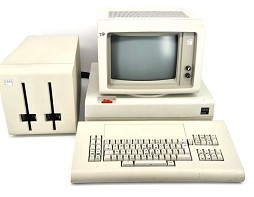
\includegraphics{./part-0/apparaetle.jpg}
\end{center}




%%%%%%%%%%%%%%%%%%%%%%%acknow.tex%%%%%%%%%%%%%%%%%%%%%%%%%%%%%%%%%%%%%%%%%
% sample acknowledgement chapter
%
% Use this file as a template for your own input.
%
%%%%%%%%%%%%%%%%%%%%%%%% Springer %%%%%%%%%%%%%%%%%%%%%%%%%%

\extrachap{Acknowledgements}

Use the template \emph{acknow.tex} together with the document class SVMono (monograph-type books) or SVMult (edited books) if you prefer to set your acknowledgement section as a separate chapter instead of including it as last part of your preface.



\tableofcontents
%%%%%%%%%%%%%%%%%%%%%clist.tex %%%%%%%%%%%%%%%%%%%%%%%%
%                                                    
% sample list of contributors and their addresses    
%                                                    
% Use this file as a template for your own input.    
%                                                    
%%%%%%%%%%%%%%%%%%%%%%%% Springer %%%%%%%%%%%%%%%%%%%%
\contributors

\begin{thecontriblist}
Firstname Surname
\at ABC Institute, 123 Prime Street, Daisy Town, NA 01234, USA, \email{smith@smith.edu}
\and
Firstname Surname
\at XYZ Institute, Technical University, Albert-Schweitzer-Str. 34, 1000 Berlin, Germany, \email{meier@tu.edu}
\end{thecontriblist}
%

\chapter{Acronyms}

\begin{description}
\item[$E_{\mathbb{R}}$, $E_{\mathbb{C}} = E$] real, complex Banach lattice
\item[$E_{+}$] positive cone
\item[$E'$] dual
\item[$E^*$] semigroup dual
\item[$E_{F}^{T}$] F-product of E with respect to semigroup T
\item[$E_{F}$] F-product of E
\item[$E_{f}$] see C-I,4
\item[$(E,\phi)$] see C-I,4
\item[$E\otimes F$] tensor product
\item[$L(E)$] bounded linear operators on E
\item[$Z(E)$] center of E
\item[$E_{n}$] n-th Sobolev space
\item[$B(H)$] W*-algebra of bounded linear operators on H
\item[$S(M)$] state space of C*-algebra M
\item[$M_{+}$] positive cone of C*-algebra M
\item[$M_{*}$] predual
\item[$M^{sa}$] self-adjoint part
\item[$M_{n}$] C*-algebra of nxn-matrices
\item[AC] absolutely continuous functions
\item[BV] functions of bounded variation
\item[K] compact topological space
\item[X] locally compact topological space
\item[$C(K)$, $C(K,E)$] continuous functions (with values in E)
\item[$C_{o}(X)$, $C_{o}(X,E)$] continuous functions vanishing at infinity with values in E
\item[$C^{b}(X)$] bounded continuous functions
\item[$C_{uu}(X)$] uniformly continuous functions
\item[$C^{n}$, $C^{(n)}$] continuous differentiable functions (n-times)
\item[$C_{c}^{\infty}(\mathbb{R}^n)$] infinitely differentiable functions with compact support
\item[$L^{p}(\mu)$] p-integrable functions
\item[$S(\mathbb{R}^n)$] Schwartz space
\item[$M(K)$] regular Borel measures
\item[$M_{b}(X)$] bounded regular Borel measures
\item[$T = (T(t))_{t\geq0}$] (one-parameter) semigroup
\item[$T|$] subspace (reduced) semigroup
\item[$T/$] quotient semigroup
\item[Fix$(T)$] fixed space of T
\item[$A$] generator
\item[$A'$] adjoint
\item[$A^*$] adjoint generator
\item[$\sigma(A)$] spectrum
\item[$\rho(A)$] resolvent set
\item[$\sigma_{ess}(A)$] essential spectrum
\item[$\sigma_{b}(A)$] boundary spectrum
\item[$P\sigma(A)$] point spectrum
\item[$P\sigma_{b}(A)$] boundary point spectrum
\item[$A\sigma(A)$] approximate point spectrum
\item[$R\sigma(A)$] residual spectrum
\item[$\omega = \omega(A) = \omega(T)$] growth bound
\item[$s(A)$] spectral bound
\item[$\omega_{I}(A)$] growth bound of solution of (ACP)
\item[$\omega(f)$] growth bound of $T(\cdot)f$
\item[$r(T)$] spectral radius
\item[$\omega_{ess}(A)$] essential growth bound
\item[$r_{ess}(T)$] essential spectral radius
\item[$R(\lambda,A)$] resolvent operator
\item[$I^{d}$, $\{I^{d}\}_{d=1}^{dd}$] orthogonal band of I (of $I^{d}$)
\item[$\wedge$] infimum
\item[$\vee$] supremum
\item[$|T|$] modulus of regular operator
\item[$\hat{f}$, $\check{f}$] Fourier (inverse Fourier) transformation
\item[$d\rho(f)$] subdifferential of $\rho$ in f
\item[$dN(f)$] subdifferential of norm in f
\item[$dN^{+}(f)$] subdifferential of canonical half-norm in f
\item[im] range
\item[ker] null-space
\item[Im] imaginary part
\item[Re] real part
\item[$\text{Re}f$, $\text{Im}f$] see C-I,7
\item[$\text{Re}T$, $\text{Im}T$] see C-I,7
\item[$\bar{f}$] complex conjugate of f
\item[$S_{f}$] signum operator with respect to f
\item[sign $f$] signum of f
\item[$f^{[n]}$] see C-II,2.2
\item[$|f|$] absolute value of f
\item[$f^{+}$] positive part of f
\item[$f^{-}$] negative part of f
\item[Id] identity operator
\item[$M_{p}$] multiplication operator
\item[1] function identically 1
\item[$1_{C}$] characteristic function of set C
\item[$\delta_{x}$] Dirac measure in x
\item[tr] trace
\item[span M] linear subspace generated by M
\item[$S(\alpha)$] sector in complex plane
\item[(ACP)] abstract Cauchy problem
\item[(P)] positive minimum principle
\item[(P')] B-II,1.21
\item[(K)] Kato's (equality) inequality
\item[(RCP)] retarded Cauchy problem
\item[(RE)] retarded equation
\item[(T)] translation property
\end{description}


\mainmatter%%%%%%%%%%%%%%%%%%%%%%%%%%%%%%%%%%%%%%%%%%%%%%%%%%%%%%%
%%%%%%%%%%%%%%%%%%%%%%part.tex%%%%%%%%%%%%%%%%%%%%%%%%%%%%%%%%%%
% 
% sample part title
%
% Use this file as a template for your own input.
%
%%%%%%%%%%%%%%%%%%%%%%%% Springer %%%%%%%%%%%%%%%%%%%%%%%%%%

\begin{partbacktext}
\part{Part Title}
\noindent Use the template \emph{part.tex} together with the document class SVMono (monograph-type books) or SVMult (edited books) to style your part title page and, if desired, a short introductory text (maximum one page) on its verso page.

\end{partbacktext}
%%%%%%%%%%%%%%%%%%%%% author.tex %%%%%%%%%%%%%%%%%%%%%%%%%%%%%%%%%%%
%
% sample root file for your "contribution" to a contributed volume
%
% Use this file as a template for your own input.
%
%%%%%%%%%%%%%%%% Springer %%%%%%%%%%%%%%%%%%%%%%%%%%%%%%%%%%%%%%%%%


%% RECOMMENDED %%%%%%%%%%%%%%%%%%%%%%%%%%%%%%%%%%%%%%%%%%%%%%%%%%%
%\documentclass[graybox]{svmult}
%
%% choose options for [] as required from the list
%% in the Reference Guide
%
%\usepackage{mathptmx}       % selects Times Roman as basic font
%\usepackage{helvet}         % selects Helvetica as sans-serif font
%\usepackage{courier}        % selects Courier as typewriter font
%\usepackage{type1cm}        % activate if the above 3 fonts are
                             % not available on your system
%
%\usepackage{makeidx}         % allows index generation
%\usepackage{graphicx}        % standard LaTeX graphics tool
%                             % when including figure files
%\usepackage{multicol}        % used for the two-column index
%\usepackage[bottom]{footmisc}% places footnotes at page bottom
%
%% see the list of further useful packages
%% in the Reference Guide
%
%\makeindex             % used for the subject index
%                       % please use the style svind.ist with
%                       % your makeindex program
%
%%%%%%%%%%%%%%%%%%%%%%%%%%%%%%%%%%%%%%%%%%%%%%%%%%%%%%%%%%%%%%%%%%%%%%%%%%%%%%%%%%%%%%%%%%
%
%\begin{document}

\title{Contribution Title}
% Use \titlerunning{Short Title} for an abbreviated version of
% your contribution title if the original one is too long
\author{Name of First Author\orcidID{0000-1111-2222-3333} and\\ Name of Second Author\orcidID{1111-2222-3333-4444}}
% Use \authorrunning{Short Title} for an abbreviated version of
% your contribution title if the original one is too long
\institute{Name of First Author \at Name, Address of Institute, \email{name@email.address}
\and Name of Second Author \at Name, Address of Institute \email{name@email.address}}
%
% Use the package "url.sty" to avoid
% problems with special characters
% used in your e-mail or web address
%
\maketitle

\abstract*{Each chapter should be preceded by an abstract (no more than 200 words) that summarizes the content. The abstract will appear \textit{online} at \url{www.SpringerLink.com} and be available with unrestricted access. This allows unregistered users to read the abstract as a teaser for the complete chapter.
Please use the 'starred' version of the \texttt{abstract} command for typesetting the text of the online abstracts (cf. source file of this chapter template \texttt{abstract}) and include them with the source files of your manuscript. Use the plain \texttt{abstract} command if the abstract is also to appear in the printed version of the book.}

\abstract{Each chapter should be preceded by an abstract (no more than 200 words) that summarizes the content. The abstract will appear \textit{online} at \url{www.SpringerLink.com} and be available with unrestricted access. This allows unregistered users to read the abstract as a teaser for the complete chapter.\newline\indent
Please use the 'starred' version of the \texttt{abstract} command for typesetting the text of the online abstracts (cf. source file of this chapter template \texttt{abstract}) and include them with the source files of your manuscript. Use the plain \texttt{abstract} command if the abstract is also to appear in the printed version of the book.}

\section{Section Heading}
\label{sec:1}
Use the template \emph{chapter.tex} together with the document class SVMono (monograph-type books) or SVMult (edited books) to style the various elements of your chapter content.

Instead of simply listing headings of different levels we recommend to let every heading be followed by at least a short passage of text. Further on please use the \LaTeX\ automatism for all your cross-references and citations. And please note that the first line of text that follows a heading is not indented, whereas the first lines of all subsequent paragraphs are.

\section{Section Heading}
\label{sec:2}
% Always give a unique label
% and use \ref{<label>} for cross-references
% and \cite{<label>} for bibliographic references
% use \sectionmark{}
% to alter or adjust the section heading in the running head
Instead of simply listing headings of different levels we recommend to let every heading be followed by at least a short passage of text. Further on please use the \LaTeX\ automatism for all your cross-references and citations.

Please note that the first line of text that follows a heading is not indented, whereas the first lines of all subsequent paragraphs are.

Use the standard \verb|equation| environment to typeset your equations, e.g.
%
\begin{equation}
a \times b = c\;,
\end{equation}
%
however, for multiline equations we recommend to use the \verb|eqnarray| environment\footnote{In physics texts please activate the class option \texttt{vecphys} to depict your vectors in \textbf{\itshape boldface-italic} type - as is customary for a wide range of physical subjects}.
\begin{eqnarray}
\left|\nabla U_{\alpha}^{\mu}(y)\right| &\le&\frac1{d-\alpha}\int
\left|\nabla\frac1{|\xi-y|^{d-\alpha}}\right|\,d\mu(\xi) =
\int \frac1{|\xi-y|^{d-\alpha+1}} \,d\mu(\xi)  \\
&=&(d-\alpha+1) \int\limits_{d(y)}^\infty
\frac{\mu(B(y,r))}{r^{d-\alpha+2}}\,dr \le (d-\alpha+1)
\int\limits_{d(y)}^\infty \frac{r^{d-\alpha}}{r^{d-\alpha+2}}\,dr
\label{eq:01}
\end{eqnarray}

\subsection{Subsection Heading}
\label{subsec:2}
Instead of simply listing headings of different levels we recommend to let every heading be followed by at least a short passage of text. Further on please use the \LaTeX\ automatism for all your cross-references\index{cross-references} and citations\index{citations} as has already been described in Sect.~\ref{sec:2}.

\begin{quotation}
Please do not use quotation marks when quoting texts! Simply use the \verb|quotation| environment -- it will automatically be rendered in line with the preferred layout.
\end{quotation}


\subsubsection{Subsubsection Heading}
Instead of simply listing headings of different levels we recommend to let every heading be followed by at least a short passage of text. Further on please use the \LaTeX\ automatism for all your cross-references and citations as has already been described in Sect.~\ref{subsec:2}, see also Fig.~\ref{fig:1}\footnote{If you copy text passages, figures, or tables from other works, you must obtain \textit{permission} from the copyright holder (usually the original publisher). Please enclose the signed permission with the manuscript. The sources\index{permission to print} must be acknowledged either in the captions, as footnotes or in a separate section of the book.}

Please note that the first line of text that follows a heading is not indented, whereas the first lines of all subsequent paragraphs are.

% For figures use
%
\begin{figure}[b]
\sidecaption
% Use the relevant command for your figure-insertion program
% to insert the figure file.
% For example, with the graphicx style use
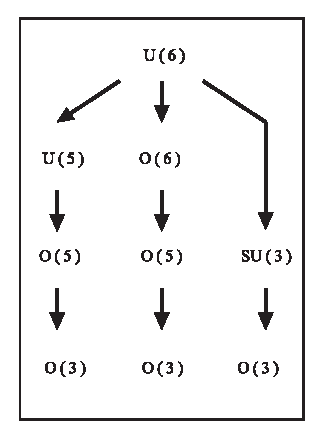
\includegraphics[scale=.65]{figure}
%
% If no graphics program available, insert a blank space i.e. use
%\picplace{5cm}{2cm} % Give the correct figure height and width in cm
%
\caption{If the width of the figure is less than 7.8 cm use the \texttt{sidecapion} command to flush the caption on the left side of the page. If the figure is positioned at the top of the page, align the sidecaption with the top of the figure -- to achieve this you simply need to use the optional argument \texttt{[t]} with the \texttt{sidecaption} command}
\label{fig:1}       % Give a unique label
\end{figure}


\paragraph{Paragraph Heading} %
Instead of simply listing headings of different levels we recommend to let every heading be followed by at least a short passage of text. Further on please use the \LaTeX\ automatism for all your cross-references and citations as has already been described in Sect.~\ref{sec:2}.

Please note that the first line of text that follows a heading is not indented, whereas the first lines of all subsequent paragraphs are.

For typesetting numbered lists we recommend to use the \verb|enumerate| environment -- it will automatically rendered in line with the preferred layout.

\begin{enumerate}
\item{Livelihood and survival mobility are oftentimes coutcomes of uneven socioeconomic development.}
\begin{enumerate}
\item{Livelihood and survival mobility are oftentimes coutcomes of uneven socioeconomic development.}
\item{Livelihood and survival mobility are oftentimes coutcomes of uneven socioeconomic development.}
\end{enumerate}
\item{Livelihood and survival mobility are oftentimes coutcomes of uneven socioeconomic development.}
\end{enumerate}


\subparagraph{Subparagraph Heading} In order to avoid simply listing headings of different levels we recommend to let every heading be followed by at least a short passage of text. Use the \LaTeX\ automatism for all your cross-references and citations as has already been described in Sect.~\ref{sec:2}, see also Fig.~\ref{fig:2}.

For unnumbered list we recommend to use the \verb|itemize| environment -- it will automatically be rendered in line with the preferred layout.

\begin{itemize}
\item{Livelihood and survival mobility are oftentimes coutcomes of uneven socioeconomic development, cf. Table~\ref{tab:1}.}
\begin{itemize}
\item{Livelihood and survival mobility are oftentimes coutcomes of uneven socioeconomic development.}
\item{Livelihood and survival mobility are oftentimes coutcomes of uneven socioeconomic development.}
\end{itemize}
\item{Livelihood and survival mobility are oftentimes coutcomes of uneven socioeconomic development.}
\end{itemize}

\begin{figure}[t]
\sidecaption[t]
% Use the relevant command for your figure-insertion program
% to insert the figure file.
% For example, with the option graphics use
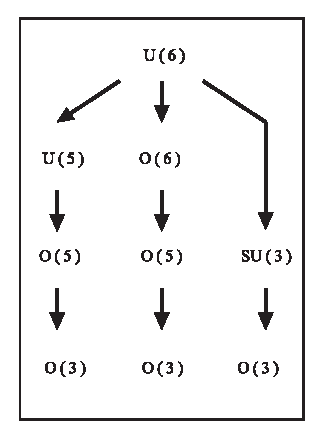
\includegraphics[scale=.65]{figure}
%
% If no graphics program available, insert a blank space i.e. use
%\picplace{5cm}{2cm} % Give the correct figure height and width in cm
%
%\caption{Please write your figure caption here}
\caption{If the width of the figure is less than 7.8 cm use the \texttt{sidecapion} command to flush the caption on the left side of the page. If the figure is positioned at the top of the page, align the sidecaption with the top of the figure -- to achieve this you simply need to use the optional argument \texttt{[t]} with the \texttt{sidecaption} command}
\label{fig:2}       % Give a unique label
\end{figure}

\runinhead{Run-in Heading Boldface Version} Use the \LaTeX\ automatism for all your cross-references and citations as has already been described in Sect.~\ref{sec:2}.

\subruninhead{Run-in Heading Boldface and Italic Version} Use the \LaTeX\ automatism for all your cross-refer\-ences and citations as has already been described in Sect.~\ref{sec:2}\index{paragraph}.

\subsubruninhead{Run-in Heading Displayed Version} Use the \LaTeX\ automatism for all your cross-refer\-ences and citations as has already been described in Sect.~\ref{sec:2}\index{paragraph}.
% Use the \index{} command to code your index words
%
% For tables use
%
\begin{table}[!t]
\caption{Please write your table caption here}
\label{tab:1}       % Give a unique label
%
% Follow this input for your own table layout
%
\begin{tabular}{p{2cm}p{2.4cm}p{2cm}p{4.9cm}}
\hline\noalign{\smallskip}
Classes & Subclass & Length & Action Mechanism  \\
\noalign{\smallskip}\svhline\noalign{\smallskip}
Translation & mRNA$^a$  & 22 (19--25) & Translation repression, mRNA cleavage\\
Translation & mRNA cleavage & 21 & mRNA cleavage\\
Translation & mRNA  & 21--22 & mRNA cleavage\\
Translation & mRNA  & 24--26 & Histone and DNA Modification\\
\noalign{\smallskip}\hline\noalign{\smallskip}
\end{tabular}
$^a$ Table foot note (with superscript)
\end{table}
%
\vspace*{-12pt}
\section{Section Heading}
\label{sec:3}
% Always give a unique label
% and use \ref{<label>} for cross-references
% and \cite{<label>} for bibliographic references
% use \sectionmark{}
% to alter or adjust the section heading in the running head
Instead of simply listing headings of different levels we recommend to let every heading be followed by at least a short passage of text. Further on please use the \LaTeX\ automatism for all your cross-references and citations as has already been described in Sect.~\ref{sec:2}.

Please note that the first line of text that follows a heading is not indented, whereas the first lines of all subsequent paragraphs are.

If you want to list definitions or the like we recommend to use the enhanced \verb|description| environment -- it will automatically rendered in line with the preferred layout.

\begin{description}[Type 1]
\item[Type 1]{That addresses central themes pertainng to migration, health, and disease. In Sect.~\ref{sec:1}, Wilson discusses the role of human migration in infectious disease distributions and patterns.}
\item[Type 2]{That addresses central themes pertainng to migration, health, and disease. In Sect.~\ref{subsec:2}, Wilson discusses the role of human migration in infectious disease distributions and patterns.}
\end{description}

\subsection{Subsection Heading} %
In order to avoid simply listing headings of different levels we recommend to let every heading be followed by at least a short passage of text. Use the \LaTeX\ automatism for all your cross-references and citations citations as has already been described in Sect.~\ref{sec:2}.

Please note that the first line of text that follows a heading is not indented, whereas the first lines of all subsequent paragraphs are.

\begin{svgraybox}
If you want to emphasize complete paragraphs of texts we recommend to use the newly defined class option \verb|graybox| and the newly defined environment \verb|svgraybox|. This will produce a 15 percent screened box 'behind' your text.

If you want to emphasize complete paragraphs of texts we recommend to use the newly defined class option and environment \verb|svgraybox|. This will produce a 15 percent screened box 'behind' your text.
\end{svgraybox}


\subsubsection{Subsubsection Heading}
Instead of simply listing headings of different levels we recommend to let every heading be followed by at least a short passage of text. Further on please use the \LaTeX\ automatism for all your cross-references and citations as has already been described in Sect.~\ref{sec:2}.

Please note that the first line of text that follows a heading is not indented, whereas the first lines of all subsequent paragraphs are.

\begin{theorem}
Theorem text goes here.
\end{theorem}
%
% or
%
\begin{definition}
Definition text goes here.
\end{definition}

\begin{proof}
%\smartqed
Proof text goes here.
%\qed
\end{proof}

\paragraph{Paragraph Heading} %
Instead of simply listing headings of different levels we recommend to let every heading be followed by at least a short passage of text. Further on please use the \LaTeX\ automatism for all your cross-references and citations as has already been described in Sect.~\ref{sec:2}.

Note that the first line of text that follows a heading is not indented, whereas the first lines of all subsequent paragraphs are.
%
% For built-in environments use
%
\begin{theorem}
Theorem text goes here.
\end{theorem}
%
\begin{definition}
Definition text goes here.
\end{definition}
%
\begin{proof}
%\smartqed
Proof text goes here.
%\qed
\end{proof}
%
\begin{trailer}{Trailer Head}
If you want to emphasize complete paragraphs of texts in an \verb|Trailer Head| we recommend to
use  \begin{verbatim}\begin{trailer}{Trailer Head}
...
\end{trailer}\end{verbatim}
\end{trailer}
%
\begin{questype}{Questions}
If you want to emphasize complete paragraphs of texts in an \verb|Questions| we recommend to
use  \begin{verbatim}\begin{questype}{Questions}
...
\end{questype}\end{verbatim}
\end{questype}

\begin{important}{Important}
If you want to emphasize complete paragraphs of texts in an \verb|Important| we recommend to
use  \begin{verbatim}\begin{important}{Important}
...
\end{important}\end{verbatim}
\end{important}
%
\eject%
\begin{warning}{Attention}
If you want to emphasize complete paragraphs of texts in an \verb|Attention| we recommend to
use  \begin{verbatim}\begin{warning}{Attention}
...
\end{warning}\end{verbatim}
\end{warning}

\begin{programcode}{Program Code}
If you want to emphasize complete paragraphs of texts in an \verb|Program Code| we recommend to
use

\verb|\begin{programcode}{Program Code}|

\verb|\begin{verbatim}...\end{verbatim}|

\verb|\end{programcode}|

\end{programcode}
%
\begin{tips}{Tips}
If you want to emphasize complete paragraphs of texts in an \verb|Tips| we recommend to
use  \begin{verbatim}\begin{tips}{Tips}
...
\end{tips}\end{verbatim}
\end{tips}

\begin{overview}{Overview}
If you want to emphasize complete paragraphs of texts in an \verb|Overview| we recommend to
use  \begin{verbatim}\begin{overview}{Overview}
...
\end{overview}\end{verbatim}
\end{overview}

\eject%
\begin{backgroundinformation}{Background Information}
If you want to emphasize complete paragraphs of texts in an \verb|Background|
\verb|Information| we recommend to
use

\verb|\begin{backgroundinformation}{Background Information}|

\verb|...|

\verb|\end{backgroundinformation}|
\end{backgroundinformation}
\begin{legaltext}{Legal Text}
If you want to emphasize complete paragraphs of texts in an \verb|Legal Text| we recommend to
use  \begin{verbatim}\begin{legaltext}{Legal Text}
...
\end{legaltext}\end{verbatim}
\end{legaltext}
%
\begin{acknowledgement}
If you want to include acknowledgments of assistance and the like at the end of an individual chapter please use the \verb|acknowledgement| environment -- it will automatically be rendered in line with the preferred layout.
\end{acknowledgement}
%
\ethics{Competing Interests}{Please declare any competing interests
in the context of your chapter. The following sentences can be regarded as examples.\newline
This study was funded by [X] [grant number X].\newline
 [Author A] has a received research grant from [Company W].\newline
 [Author B] has received a speaker honorarium from [Company X] and owns stock in [Company~Y].\newline 
 [Author C] is a member of [committee Z].\newline 
The authors have no conflicts of interest to declare that are relevant to the content of this chapter.}

\ethics{Ethics Approval}{If your chapter includes primary studies with humans please declare the adherence of ethical standards. Example text: This study was performed in line with the principles of the Declaration of Helsinki. Approval was granted by the Ethics Committee of University B (Date.../No. ...).\newline 
 In addition, for human participants, authors are required to include a statement that informed consent (to participate and/or to publish) was obtained from individual participants or parents/guardians if the participant is minor or incapable.\newline
If animals are studied, authors should make sure that the legal requirements or guidelines in the country and/or state or province for the care and use of animals have been followed or specify that no ethics approval was required.}

\eject

\section*{Appendix}
%\addcontentsline{toc}{section}{Appendix}
%
%
When placed at the end of a chapter or contribution (as opposed to at the end of the book), the numbering of tables, figures, and equations in the appendix section continues on from that in the main text. Hence please \textit{do not} use the \verb|appendix| command when writing an appendix at the end of your chapter or contribution. If there is only one the appendix is designated ``Appendix'', or ``Appendix 1'', or ``Appendix 2'', etc. if there is more than one.

\begin{equation}
a \times b = c
\end{equation}

%%%%%%%%%%%%%%%%%%%%%%%% referenc.tex %%%%%%%%%%%%%%%%%%%%%%%%%%%%%%
% sample references
% %
% Use this file as a template for your own input.
%
%%%%%%%%%%%%%%%%%%%%%%%% Springer-Verlag %%%%%%%%%%%%%%%%%%%%%%%%%%
%
% BibTeX users please use
% \bibliographystyle{}
% \bibliography{}
%
%\biblstarthook{
\section{Styling of References}
In view of the parallel print and (chapter-wise) online publication of your book at \url{www.springerlink.com} it has been decided that -- as a genreral rule --  references should be sorted chapter-wise and placed at the end of the individual chapters. However, upon agreement with your contact at Springer you may list your references in a single seperate chapter at the end of your book. Deactivate the class option \texttt{sectrefs} and the \texttt{thebibliography} environment will be put out as a chapter of its own.\\\indent
References may be \textit{cited} in the text either by number (preferred) or by author/year.\footnote{Make sure that all references from the list are cited in the text. Those not cited should be moved to a separate \textit{Further Reading} section or chapter.} If the citatiion in the text is numbered, the reference list should be arranged in ascending order. If the citation in the text is author/year, the reference list should be \textit{sorted} alphabetically and if there are several works by the same author, the following order should be used:
\begin{enumerate}
\item all works by the author alone, ordered chronologically by year of publication
\item all works by the author with a coauthor, ordered alphabetically by coauthor
\item all works by the author with several coauthors, ordered chronologically by year of publication.
\end{enumerate}
The \textit{styling} of references\footnote{Always use the standard abbreviation of a journal's name according to the ISSN \textit{List of Title Word Abbreviations}, see \url{http://www.issn.org/en/node/344}} depends on the subject of your book:
\begin{itemize}
\item The \textit{two} recommended styles for references in books on \textit{mathematical, physical, statistical and computer sciences} are depicted in ~\cite{science-contrib, science-online, science-mono, science-journal, science-DOI} and ~\cite{phys-online, phys-mono, phys-journal, phys-DOI, phys-contrib}.
\item Examples of the most commonly used reference style in books on \textit{Psychology, Social Sciences} are~\cite{psysoc-mono, psysoc-online,psysoc-journal, psysoc-contrib, psysoc-DOI}.
\item Examples for references in books on \textit{Humanities, Linguistics, Philosophy} are~\cite{humlinphil-journal, humlinphil-contrib, humlinphil-mono, humlinphil-online, humlinphil-DOI}.
\item Examples of the basic Springer style used in publications on a wide range of subjects such as \textit{Computer Science, Economics, Engineering, Geosciences, Life Sciences, Medicine, Biomedicine} are ~\cite{basic-contrib, basic-online, basic-journal, basic-DOI, basic-mono}. 
\end{itemize}
%}

\begin{thebibliography}{99.}%
% and use \bibitem to create references.
%
% Use the following syntax and markup for your references if 
% the subject of your book is from the field 
% "Mathematics, Physics, Statistics, Computer Science"
%
% Contribution 
\bibitem{science-contrib} Broy, M.: Software engineering --- from auxiliary to key technologies. In: Broy, M., Dener, E. (eds.) Software Pioneers, pp. 10-13. Springer, Heidelberg (2002)
%
% Online Document
\bibitem{science-online} Dod, J.: Effective substances. In: The Dictionary of Substances and Their Effects. Royal Society of Chemistry (1999) Available via DIALOG. \\
\url{http://www.rsc.org/dose/title of subordinate document. Cited 15 Jan 1999}
%
% Monograph
\bibitem{science-mono} Geddes, K.O., Czapor, S.R., Labahn, G.: Algorithms for Computer Algebra. Kluwer, Boston (1992) 
%
% Journal article
\bibitem{science-journal} Hamburger, C.: Quasimonotonicity, regularity and duality for nonlinear systems of partial differential equations. Ann. Mat. Pura. Appl. \textbf{169}, 321--354 (1995)
%
% Journal article by DOI
\bibitem{science-DOI} Slifka, M.K., Whitton, J.L.: Clinical implications of dysregulated cytokine production. J. Mol. Med. (2000) doi: 10.1007/s001090000086 
%
%\bigskip

% Use the following (APS) syntax and markup for your references if 
% the subject of your book is from the field 
% "Mathematics, Physics, Statistics, Computer Science"
%
% Online Document
\bibitem{phys-online} J. Dod, in \textit{The Dictionary of Substances and Their Effects}, Royal Society of Chemistry. (Available via DIALOG, 1999), 
\url{http://www.rsc.org/dose/title of subordinate document. Cited 15 Jan 1999}
%
% Monograph
\bibitem{phys-mono} H. Ibach, H. L\"uth, \textit{Solid-State Physics}, 2nd edn. (Springer, New York, 1996), pp. 45-56 
%
% Journal article
\bibitem{phys-journal} S. Preuss, A. Demchuk Jr., M. Stuke, Appl. Phys. A \textbf{61}
%
% Journal article by DOI
\bibitem{phys-DOI} M.K. Slifka, J.L. Whitton, J. Mol. Med., doi: 10.1007/s001090000086
%
% Contribution 
\bibitem{phys-contrib} S.E. Smith, in \textit{Neuromuscular Junction}, ed. by E. Zaimis. Handbook of Experimental Pharmacology, vol 42 (Springer, Heidelberg, 1976), p. 593
%
%\bigskip
%
% Use the following syntax and markup for your references if 
% the subject of your book is from the field 
% "Psychology, Social Sciences"
%
%
% Monograph
\bibitem{psysoc-mono} Calfee, R.~C., \& Valencia, R.~R. (1991). \textit{APA guide to preparing manuscripts for journal publication.} Washington, DC: American Psychological Association.
%
% Online Document
\bibitem{psysoc-online} Dod, J. (1999). Effective substances. In: The dictionary of substances and their effects. Royal Society of Chemistry. Available via DIALOG. \\
\url{http://www.rsc.org/dose/Effective substances.} Cited 15 Jan 1999.
%
% Journal article
\bibitem{psysoc-journal} Harris, M., Karper, E., Stacks, G., Hoffman, D., DeNiro, R., Cruz, P., et al. (2001). Writing labs and the Hollywood connection. \textit{J Film} Writing, 44(3), 213--245.
%
% Contribution 
\bibitem{psysoc-contrib} O'Neil, J.~M., \& Egan, J. (1992). Men's and women's gender role journeys: Metaphor for healing, transition, and transformation. In B.~R. Wainrig (Ed.), \textit{Gender issues across the life cycle} (pp. 107--123). New York: Springer.
%
% Journal article by DOI
\bibitem{psysoc-DOI}Kreger, M., Brindis, C.D., Manuel, D.M., Sassoubre, L. (2007). Lessons learned in systems change initiatives: benchmarks and indicators. \textit{American Journal of Community Psychology}, doi: 10.1007/s10464-007-9108-14.
%
%
% Use the following syntax and markup for your references if 
% the subject of your book is from the field 
% "Humanities, Linguistics, Philosophy"
%
%\bigskip
%
% Journal article
\bibitem{humlinphil-journal} Alber John, Daniel C. O'Connell, and Sabine Kowal. 2002. Personal perspective in TV interviews. \textit{Pragmatics} 12:257--271
%
% Contribution 
\bibitem{humlinphil-contrib} Cameron, Deborah. 1997. Theoretical debates in feminist linguistics: Questions of sex and gender. In \textit{Gender and discourse}, ed. Ruth Wodak, 99--119. London: Sage Publications.
%
% Monograph
\bibitem{humlinphil-mono} Cameron, Deborah. 1985. \textit{Feminism and linguistic theory.} New York: St. Martin's Press.
%
% Online Document
\bibitem{humlinphil-online} Dod, Jake. 1999. Effective substances. In: The dictionary of substances and their effects. Royal Society of Chemistry. Available via DIALOG. \\
http://www.rsc.org/dose/title of subordinate document. Cited 15 Jan 1999
%
% Journal article by DOI
\bibitem{humlinphil-DOI} Suleiman, Camelia, Daniel C. O'Connell, and Sabine Kowal. 2002. `If you and I, if we, in this later day, lose that sacred fire...': Perspective in political interviews. \textit{Journal of Psycholinguistic Research}. doi: 10.1023/A:1015592129296.
%
%
%
%\bigskip
%
%
% Use the following syntax and markup for your references if 
% the subject of your book is from the field 
% "Computer Science, Economics, Engineering, Geosciences, Life Sciences"
%
%
% Contribution 
\bibitem{basic-contrib} Brown B, Aaron M (2001) The politics of nature. In: Smith J (ed) The rise of modern genomics, 3rd edn. Wiley, New York 
%
% Online Document
\bibitem{basic-online} Dod J (1999) Effective Substances. In: The dictionary of substances and their effects. Royal Society of Chemistry. Available via DIALOG. \\
\url{http://www.rsc.org/dose/title of subordinate document. Cited 15 Jan 1999}
%
% Journal article by DOI
\bibitem{basic-DOI} Slifka MK, Whitton JL (2000) Clinical implications of dysregulated cytokine production. J Mol Med, doi: 10.1007/s001090000086
%
% Journal article
\bibitem{basic-journal} Smith J, Jones M Jr, Houghton L et al (1999) Future of health insurance. N Engl J Med 965:325--329
%
% Monograph
\bibitem{basic-mono} South J, Blass B (2001) The future of modern genomics. Blackwell, London 
%
\end{thebibliography}

%\end{document}

%

\backmatter%%%%%%%%%%%%%%%%%%%%%%%%%%%%%%%%%%%%%%%%%%%%%%%%%%%%%%%
\appendix
%%%%%%%%%%%%%%%%%%%%%% appendix.tex %%%%%%%%%%%%%%%%%%%%%%%%%%%%%%%%%
%
% sample appendix
%
% Use this file as a template for your own input.
%
%%%%%%%%%%%%%%%%%%%%%%%% Springer-Verlag %%%%%%%%%%%%%%%%%%%%%%%%%%

\chapter{Chapter Heading}
\label{introA} % Always give a unique label
% use \chaptermark{}
% to alter or adjust the chapter heading in the running head

Use the template \emph{appendix.tex} together with the document class SVMono (monograph-type books) or SVMult (edited books) to style appendix of your book.


\section{Section Heading}
\label{sec:A1}
% Always give a unique label
% and use \ref{<label>} for cross-references
% and \cite{<label>} for bibliographic references
% use \sectionmark{}
% to alter or adjust the section heading in the running head
Instead of simply listing headings of different levels we recommend to let every heading be followed by at least a short passage of text. Further on please use the \LaTeX\ automatism for all your cross-references and citations.


\subsection{Subsection Heading}
\label{sec:A2}
Instead of simply listing headings of different levels we recommend to let every heading be followed by at least a short passage of text. Further on please use the \LaTeX\ automatism for all your cross-references and citations as has already been described in Sect.~\ref{sec:A1}.

For multiline equations we recommend to use the \verb|eqnarray| environment.
\begin{eqnarray}
\vec{a}\times\vec{b}=\vec{c} \nonumber\\
\vec{a}\times\vec{b}=\vec{c}
\label{eq:A01}
\end{eqnarray}

\subsubsection{Subsubsection Heading}
Instead of simply listing headings of different levels we recommend to let every heading be followed by at least a short passage of text. Further on please use the \LaTeX\ automatism for all your cross-references and citations as has already been described in Sect.~\ref{sec:A2}.

Please note that the first line of text that follows a heading is not indented, whereas the first lines of all subsequent paragraphs are.

% For figures use
%
\begin{figure}[t]
\sidecaption[t]
% Use the relevant command for your figure-insertion program
% to insert the figure file.
% For example, with the graphicx style use
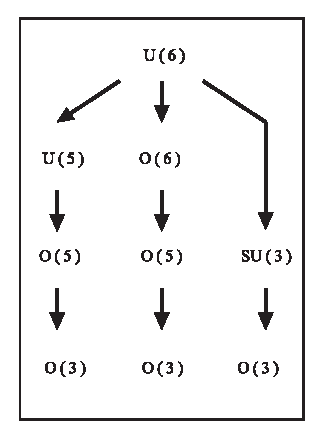
\includegraphics[scale=.65]{figure}
%
% If no graphics program available, insert a blank space i.e. use
%\picplace{5cm}{2cm} % Give the correct figure height and width in cm
%
\caption{Please write your figure caption here}
\label{fig:A1}       % Give a unique label
\end{figure}

% For tables use
%
\begin{table}
\caption{Please write your table caption here}
\label{tab:A1}       % Give a unique label
%
% Follow this input for your own table layout
%
\begin{tabular}{p{2cm}p{2.4cm}p{2cm}p{4.9cm}}
\hline\noalign{\smallskip}
Classes & Subclass & Length & Action Mechanism  \\
\noalign{\smallskip}\hline\noalign{\smallskip}
Translation & mRNA$^a$  & 22 (19--25) & Translation repression, mRNA cleavage\\
Translation & mRNA cleavage & 21 & mRNA cleavage\\
Translation & mRNA  & 21--22 & mRNA cleavage\\
Translation & mRNA  & 24--26 & Histone and DNA Modification\\
\noalign{\smallskip}\hline\noalign{\smallskip}
\end{tabular}
$^a$ Table foot note (with superscript)
\end{table}
%

%%%%%%%%%%%%%%%%%%%%%%%acronym.tex%%%%%%%%%%%%%%%%%%%%%%%%%%%%%%%%%%%%%%%%%
% sample list of acronyms
%
% Use this file as a template for your own input.
%
%%%%%%%%%%%%%%%%%%%%%%%% Springer Nature%%%%%%%%%%%%%%%%%%%%%%%%%%

\Extrachap{Glossary}


Use the template \emph{glossary.tex} together with the Springer Nature document class SVMono (monograph-type books) or SVMult (edited books) to style your glossary\index{glossary} in the Springer Nature layout.


\runinhead{glossary term} Write here the description of the glossary term. Write here the description of the glossary term. Write here the description of the glossary term.

\runinhead{glossary term} Write here the description of the glossary term. Write here the description of the glossary term. Write here the description of the glossary term.

\runinhead{glossary term} Write here the description of the glossary term. Write here the description of the glossary term. Write here the description of the glossary term.

\runinhead{glossary term} Write here the description of the glossary term. Write here the description of the glossary term. Write here the description of the glossary term.

\runinhead{glossary term} Write here the description of the glossary term. Write here the description of the glossary term. Write here the description of the glossary term.
%\printindex

%%%%%%%%%%%%%%%%%%%%%%%%%%%%%%%%%%%%%%%%%%%%%%%%%%%%%%%%%%%%%%%%%%%%%%

\end{document}

